\documentclass[12pt,a4paper]{article}

% ================================================================
%  Factorial Walkthrough -- PLC Language
% ================================================================

\usepackage{amsmath,amssymb}
\usepackage{graphicx}
\usepackage{float}
\usepackage{booktabs}
\usepackage{enumitem}
\usepackage[T1]{fontenc}
\usepackage[utf8]{inputenc}
\usepackage{listings}
\usepackage{tcolorbox}
\usepackage{caption}
\usepackage{array}
\usepackage{longtable}

% ---- Times New Roman ----
\usepackage{mathptmx}

% ---- A4, 1 inch all margins ----
\usepackage[a4paper,
            top=1in, bottom=1in, left=1in, right=1in,
            headheight=14pt, headsep=0.2in, footskip=0.3in]{geometry}

% ---- 1.5x line spacing ----
\usepackage{setspace}
\setstretch{1.5}

\setlength{\parindent}{0pt}
\setlength{\parskip}{6pt}
\setlength{\emergencystretch}{2em}
\hbadness=10000
\hfuzz=5pt

% ---- Colours ----
\usepackage[table]{xcolor}
\definecolor{codebg}{RGB}{248,248,248}
\definecolor{codeframe}{RGB}{200,200,200}
\definecolor{keyword}{RGB}{0,0,180}
\definecolor{comment}{RGB}{0,128,0}
\definecolor{string}{RGB}{163,21,21}
\definecolor{boxblue}{RGB}{220,235,250}
\definecolor{boxgreen}{RGB}{210,245,220}
\definecolor{boxorange}{RGB}{255,235,210}
\definecolor{rowgray}{RGB}{245,245,245}

% ---- TikZ ----
\usepackage{tikz}
\usetikzlibrary{shapes.geometric, arrows.meta, positioning, fit,
                backgrounds, calc, decorations.pathreplacing}

\usepackage{hyperref}
\hypersetup{colorlinks=false, hidelinks}

% ---- Code listings ----
\lstdefinelanguage{PLC}{
  morekeywords={def, if, else, while, return, true, false, print},
  sensitive=true,
  morestring=[b]",
  morecomment=[l]{//},
}

\lstset{
  language=PLC,
  basicstyle=\footnotesize\ttfamily,
  keywordstyle=\color{keyword}\bfseries,
  commentstyle=\color{comment}\itshape,
  stringstyle=\color{string},
  columns=fullflexible,
  breaklines=true,
  lineskip=0.4ex,
  frame=single,
  backgroundcolor=\color{codebg},
  rulecolor=\color{codeframe},
  numbers=left,
  numberstyle=\tiny\color{gray},
  numbersep=8pt,
  showstringspaces=false,
  tabsize=4,
  captionpos=b,
}

\tcbuselibrary{skins,breakable}

\newtcolorbox{stagebox}[2][]{
  colback=boxblue,
  colframe=blue!40!black,
  fonttitle=\bfseries,
  title={#2},
  #1
}

\newtcolorbox{notebox}[1][]{
  colback=boxorange,
  colframe=orange!60!black,
  fonttitle=\bfseries,
  #1
}

% ---- Page numbers ----
\usepackage{fancyhdr}
\pagestyle{fancy}
\fancyhf{}
\renewcommand{\headrulewidth}{0pt}
\fancyfoot[C]{\thepage}

% ================================================================
\begin{document}

\begin{titlepage}
  \centering
  \vspace*{1.5cm}
  {\Large\bfseries PLC Language --- Factorial Processing Walkthrough\par}
  \vspace{0.5cm}
  {\large A Step-by-Step Trace Through the Compiler Pipeline\par}
  \vspace{2cm}
  {\normalsize
    This document traces the complete execution of an iterative factorial
    program through every stage of the PLC language pipeline: lexical
    analysis, parsing, type checking, and tree-walking interpretation.
    The program computes \texttt{factorial(5) = 120}.
  \par}
  \vspace{3cm}
  {\normalsize May 2026\par}
\end{titlepage}

\tableofcontents
\newpage

% ================================================================
\section{The Source Program}

The program used throughout this walkthrough is the iterative factorial
implementation from \texttt{demos/demo\_11\_full.txt}.
Recursion is not supported by the type checker, so factorial is computed
using an accumulator variable inside a \texttt{while} loop.

\begin{lstlisting}[caption={Iterative factorial program (demo\_11\_full.txt, lines 1--19)},label={lst:source}]
def factorial(n) {
    result = 1;
    i = n;
    while (i != 0) {
        result = result * i;
        i = i - 1;
    }
    return result;
}

x = 5;
f = factorial(x);
print(f);
\end{lstlisting}

The pipeline processes this source through four sequential stages,
each described in its own section below.

\begin{figure}[H]
  \centering
  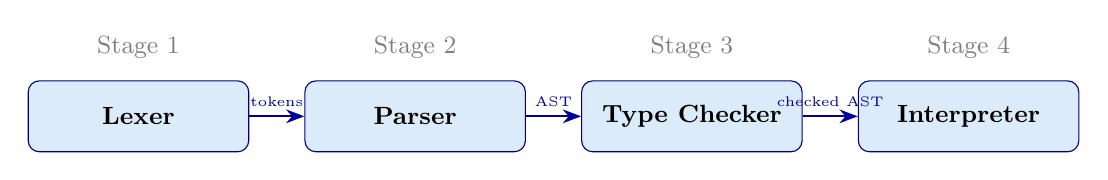
\begin{tikzpicture}[
      box/.style={rectangle, rounded corners=4pt, minimum width=2.8cm,
                  minimum height=0.9cm, text centered, font=\small\bfseries,
                  draw=blue!50!black, fill=boxblue},
      arr/.style={-Stealth, thick, color=blue!60!black},
      node distance=0.7cm
    ]
    \node[box] (lex)   {Lexer};
    \node[box, right=of lex]  (par)   {Parser};
    \node[box, right=of par]  (tc)    {Type Checker};
    \node[box, right=of tc]   (interp){Interpreter};

    \draw[arr] (lex)    -- node[above,font=\tiny]{tokens}     (par);
    \draw[arr] (par)    -- node[above,font=\tiny]{AST}         (tc);
    \draw[arr] (tc)     -- node[above,font=\tiny]{checked AST} (interp);

    \node[font=\small, above=0.15cm of lex, text=gray]   {Stage 1};
    \node[font=\small, above=0.15cm of par, text=gray]   {Stage 2};
    \node[font=\small, above=0.15cm of tc,  text=gray]   {Stage 3};
    \node[font=\small, above=0.15cm of interp, text=gray]{Stage 4};
  \end{tikzpicture}
  \caption{The four-stage PLC compiler pipeline.}
\end{figure}

% ================================================================
\section{Stage 1 --- Lexical Analysis}

\subsection{Role of the Lexer}

The lexer (\texttt{components/lexica.py}) scans the raw source text
character by character and groups characters into \emph{tokens}.
Each token has a \emph{type} (from the \texttt{TokenType} enum in
\texttt{components/tokens.py}), a \emph{lexeme} (the exact text matched),
and a \emph{line} and \emph{column} position for error reporting.
Whitespace and newlines are consumed but not emitted as tokens.

\subsection{Token Stream Produced}

Table~\ref{tab:tokens} shows the complete token stream for the factorial
program.  Tokens are listed in the order the lexer emits them.

\begin{longtable}{@{}lll@{}}
  \caption{Token stream for the factorial program.}\label{tab:tokens}\\
  \toprule
  \textbf{Token type} & \textbf{Lexeme} & \textbf{Notes} \\
  \midrule
  \endfirsthead
  \toprule
  \textbf{Token type} & \textbf{Lexeme} & \textbf{Notes} \\
  \midrule
  \endhead
  \bottomrule
  \endfoot
  % --- function definition ---
  \rowcolor{rowgray}
  \texttt{DEF}        & \texttt{def}       & Keyword \\
  \texttt{IDENTIFIER} & \texttt{factorial} & Function name \\
  \rowcolor{rowgray}
  \texttt{LPAREN}     & \texttt{(}         & \\
  \texttt{IDENTIFIER} & \texttt{n}         & Parameter name \\
  \rowcolor{rowgray}
  \texttt{RPAREN}     & \texttt{)}         & \\
  \texttt{LBRACE}     & \texttt{\{}        & Begin function body \\
  % --- result = 1 ---
  \rowcolor{rowgray}
  \texttt{IDENTIFIER} & \texttt{result}    & \\
  \texttt{ASSIGN}     & \texttt{=}         & \\
  \rowcolor{rowgray}
  \texttt{INT}        & \texttt{1}         & Integer literal \\
  \texttt{SEMICOLON}  & \texttt{;}         & \\
  % --- i = n ---
  \rowcolor{rowgray}
  \texttt{IDENTIFIER} & \texttt{i}         & \\
  \texttt{ASSIGN}     & \texttt{=}         & \\
  \rowcolor{rowgray}
  \texttt{IDENTIFIER} & \texttt{n}         & \\
  \texttt{SEMICOLON}  & \texttt{;}         & \\
  % --- while ---
  \rowcolor{rowgray}
  \texttt{WHILE}      & \texttt{while}     & Keyword \\
  \texttt{LPAREN}     & \texttt{(}         & \\
  \rowcolor{rowgray}
  \texttt{IDENTIFIER} & \texttt{i}         & \\
  \texttt{BANG\_EQUAL}& \texttt{!=}        & Not-equal operator \\
  \rowcolor{rowgray}
  \texttt{INT}        & \texttt{0}         & Integer literal \\
  \texttt{RPAREN}     & \texttt{)}         & \\
  \rowcolor{rowgray}
  \texttt{LBRACE}     & \texttt{\{}        & Begin loop body \\
  % --- result = result * i ---
  \texttt{IDENTIFIER} & \texttt{result}    & \\
  \rowcolor{rowgray}
  \texttt{ASSIGN}     & \texttt{=}         & \\
  \texttt{IDENTIFIER} & \texttt{result}    & \\
  \rowcolor{rowgray}
  \texttt{STAR}       & \texttt{*}         & Integer multiply \\
  \texttt{IDENTIFIER} & \texttt{i}         & \\
  \rowcolor{rowgray}
  \texttt{SEMICOLON}  & \texttt{;}         & \\
  % --- i = i - 1 ---
  \texttt{IDENTIFIER} & \texttt{i}         & \\
  \rowcolor{rowgray}
  \texttt{ASSIGN}     & \texttt{=}         & \\
  \texttt{IDENTIFIER} & \texttt{i}         & \\
  \rowcolor{rowgray}
  \texttt{MINUS}      & \texttt{-}         & Integer subtract \\
  \texttt{INT}        & \texttt{1}         & Integer literal \\
  \rowcolor{rowgray}
  \texttt{SEMICOLON}  & \texttt{;}         & \\
  % --- close while body ---
  \texttt{RBRACE}     & \texttt{\}}        & End loop body \\
  % --- return result ---
  \rowcolor{rowgray}
  \texttt{RETURN}     & \texttt{return}    & Keyword \\
  \texttt{IDENTIFIER} & \texttt{result}    & \\
  \rowcolor{rowgray}
  \texttt{SEMICOLON}  & \texttt{;}         & \\
  % --- close function ---
  \texttt{RBRACE}     & \texttt{\}}        & End function body \\
  % --- x = 5 ---
  \rowcolor{rowgray}
  \texttt{IDENTIFIER} & \texttt{x}         & \\
  \texttt{ASSIGN}     & \texttt{=}         & \\
  \rowcolor{rowgray}
  \texttt{INT}        & \texttt{5}         & Integer literal \\
  \texttt{SEMICOLON}  & \texttt{;}         & \\
  % --- f = factorial(x) ---
  \rowcolor{rowgray}
  \texttt{IDENTIFIER} & \texttt{f}         & \\
  \texttt{ASSIGN}     & \texttt{=}         & \\
  \rowcolor{rowgray}
  \texttt{IDENTIFIER} & \texttt{factorial} & Callee name \\
  \texttt{LPAREN}     & \texttt{(}         & \\
  \rowcolor{rowgray}
  \texttt{IDENTIFIER} & \texttt{x}         & Argument \\
  \texttt{RPAREN}     & \texttt{)}         & \\
  \rowcolor{rowgray}
  \texttt{SEMICOLON}  & \texttt{;}         & \\
  % --- print(f) ---
  \texttt{IDENTIFIER} & \texttt{print}     & Built-in function \\
  \rowcolor{rowgray}
  \texttt{LPAREN}     & \texttt{(}         & \\
  \texttt{IDENTIFIER} & \texttt{f}         & \\
  \rowcolor{rowgray}
  \texttt{RPAREN}     & \texttt{)}         & \\
  \texttt{SEMICOLON}  & \texttt{;}         & \\
  \rowcolor{rowgray}
  \texttt{EOF}        & \textit{(end)}     & Signals end of input \\
\end{longtable}

\subsection{Key Lexer Decisions}

\begin{itemize}[noitemsep]
  \item \textbf{Keyword vs.\ identifier.}  The lexer first reads a run of
    alphanumeric characters and underscores, then checks a keyword map.
    \texttt{def}, \texttt{while}, and \texttt{return} are emitted as their
    own keyword tokens; \texttt{factorial}, \texttt{n}, \texttt{result},
    \texttt{i}, \texttt{x}, and \texttt{f} are emitted as \texttt{IDENTIFIER}.

  \item \textbf{Integer vs.\ float literals.}  A sequence of digits without a
    decimal point is emitted as \texttt{INT}; a sequence containing a decimal
    point is emitted as \texttt{FLOAT}.  No float literals appear in this
    program.

  \item \textbf{Float operators vs.\ integer operators.}  The lexer
    distinguishes \texttt{*} (\texttt{STAR}) from \texttt{*.}
    (\texttt{STAR\_DOT}) and \texttt{-} (\texttt{MINUS}) from \texttt{-.}
    (\texttt{MINUS\_DOT}).  Only integer operators appear here.

  \item \textbf{\texttt{!=} two-character token.}  The lexer reads
    \texttt{!} and peeks ahead: if the next character is \texttt{=} it
    consumes both and emits \texttt{BANG\_EQUAL}.
\end{itemize}

% ================================================================
\section{Stage 2 --- Parsing}

\subsection{Role of the Parser}

The parser (\texttt{components/parser.py}) is a hand-written
recursive-descent parser.  It consumes the token stream produced by the
lexer and constructs an \emph{Abstract Syntax Tree} (AST) whose nodes are
dataclasses defined in \texttt{components/ast\_nodes.py}.  The root node
is always a \texttt{Program}, which holds a flat list of top-level
statements.

\subsection{AST Produced}

The parser produces the following tree for the factorial program.
Indentation represents parent--child relationships.

\begin{lstlisting}[language={},numbers=none,frame=none,
  backgroundcolor=\color{white},
  caption={Abstract Syntax Tree for the factorial program.}]
Program
  FunctionDef  name="factorial"  params=["n"]
    Block
      Assign  name="result"
        Literal  value=1  (Integer)
      Assign  name="i"
        Identifier  name="n"
      While
        BinaryOp  op="!="
          Identifier  name="i"
          Literal  value=0  (Integer)
        Block  (loop body)
          Assign  name="result"
            BinaryOp  op="*"
              Identifier  name="result"
              Identifier  name="i"
          Assign  name="i"
            BinaryOp  op="-"
              Identifier  name="i"
              Literal  value=1  (Integer)
      Return
        Identifier  name="result"
  Assign  name="x"
    Literal  value=5  (Integer)
  Assign  name="f"
    FunctionCall  name="factorial"
      Identifier  name="x"
  FunctionCall  name="print"
    Identifier  name="f"
\end{lstlisting}

\subsection{How Each Construct is Parsed}

\subsubsection{Function Definition}

When the parser sees a \texttt{DEF} token it enters
\texttt{\_parse\_func\_def()}.  It reads the function name, the
comma-separated parameter list between parentheses, and then calls
\texttt{\_parse\_block()} to consume the body enclosed in braces.  The
result is a \texttt{FunctionDef} node.  No type annotations are written
by the programmer; all type information is inferred later.

\subsubsection{While Statement}

On encountering \texttt{WHILE} the parser reads the condition expression
between parentheses, then calls \texttt{\_parse\_block()} for the loop
body.  The condition \texttt{i != 0} is parsed as a comparison expression:
first \texttt{i} is parsed as an \texttt{Identifier}, then \texttt{!=}
is consumed, then \texttt{0} is parsed as an integer \texttt{Literal},
and together they form \texttt{BinaryOp(op="!=", left=Identifier("i"),
right=Literal(0))}.

\subsubsection{Assignment}

A statement that starts with an \texttt{IDENTIFIER} followed by
\texttt{ASSIGN} is parsed as an \texttt{Assign} node.  For example,
\texttt{result = result * i} becomes \texttt{Assign(name="result",
value=BinaryOp("*", Identifier("result"), Identifier("i")))}.

\subsubsection{Function Call}

An \texttt{IDENTIFIER} immediately followed by \texttt{LPAREN} is parsed
as a \texttt{FunctionCall}.  The argument list between the parentheses is
parsed as a comma-separated sequence of expressions.  For
\texttt{factorial(x)}, the single argument \texttt{x} is parsed as
\texttt{Identifier("x")}.

\subsubsection{Expression Precedence}

The grammar implements standard arithmetic precedence through three levels
of recursive-descent rules:

\begin{center}
\begin{tabular}{ll}
  \toprule
  \textbf{Rule} & \textbf{Handles} \\
  \midrule
  \texttt{\_expr()}    & Comparison (\texttt{==}, \texttt{!=}) \\
  \texttt{\_additive()} & Addition and subtraction (\texttt{+}, \texttt{-}, \texttt{+.}, \texttt{-.}) \\
  \texttt{\_term()}     & Multiplication and division (\texttt{*}, \texttt{/}, \texttt{*.}, \texttt{/.}) \\
  \texttt{\_factor()}   & Literals, identifiers, calls, grouped expressions \\
  \bottomrule
\end{tabular}
\end{center}

% ================================================================
\section{Stage 3 --- Type Checking}

\subsection{Role of the Type Checker}

The type checker (\texttt{components/type\_checker.py}) performs a
single-pass, syntax-directed traversal of the AST.  Its goals are:

\begin{enumerate}[noitemsep]
  \item Build a \emph{symbol table} mapping every variable and function
    name to its inferred type.
  \item Verify that every operator is applied to operands of the correct
    type.
  \item Verify that \texttt{while} and \texttt{if} conditions are
    \texttt{Boolean}.
  \item Infer the parameter and return types of user-defined functions
    from their usage context.
  \item Reject recursive function calls.
\end{enumerate}

No type annotations are required from the programmer.  Types are inferred
entirely from context.

\subsection{Two-Pass Function Registration}

Before checking any expression or statement, the type checker makes a
preliminary scan of the top-level statement list.  Any
\texttt{FunctionDef} node is registered in the symbol table as a
\texttt{FunctionSymbol} with \emph{placeholder} (unknown) parameter types.
This ensures that a function can be referenced before its call site is
seen.

\subsection{Checking the Top-Level Statements}

\subsubsection{Statement: \texttt{x = 5}}

The right-hand side is \texttt{Literal(5)}.  The literal's value is the
Python integer \texttt{5}, so its type is \texttt{Integer}.  The type
checker records \texttt{x : Integer} in the global symbol table.

\subsubsection{Statement: \texttt{f = factorial(x)}}

The right-hand side is \texttt{FunctionCall("factorial", [Identifier("x")])}.
The type checker:

\begin{enumerate}[noitemsep]
  \item Looks up \texttt{x} in the symbol table: \texttt{Integer}.
  \item This is the \emph{first call} to \texttt{factorial}, so the
    placeholder parameter type for \texttt{n} is fixed to \texttt{Integer}.
  \item The function body is now type-checked with \texttt{n : Integer}
    in scope (inside a dedicated function scope).  The name \texttt{factorial}
    is pushed onto \texttt{\_active\_calls} to detect recursion.
  \item The body checking proceeds (detailed in the next subsection).
  \item The inferred return type of \texttt{factorial} is \texttt{Integer}.
  \item \texttt{f : Integer} is recorded in the global symbol table.
\end{enumerate}

\subsubsection{Checking the Function Body}

With \texttt{n : Integer} in the function scope:

\begin{center}
\begin{tabular}{p{5cm}p{2.5cm}p{5cm}}
  \toprule
  \textbf{Statement} & \textbf{Inferred type} & \textbf{Action} \\
  \midrule
  \texttt{result = 1}
    & \texttt{Integer}
    & Record \texttt{result : Integer} in function scope. \\[4pt]
  \texttt{i = n}
    & \texttt{Integer}
    & Look up \texttt{n}: \texttt{Integer}. Record \texttt{i : Integer}. \\[4pt]
  \texttt{while (i != 0)}~condition
    & \texttt{Boolean}
    & Both operands \texttt{i} and \texttt{0} are \texttt{Integer};
      \texttt{!=} on integers yields \texttt{Boolean}.  Condition is
      \texttt{Boolean}: pass. \\[4pt]
  \texttt{result = result * i}
    & \texttt{Integer}
    & Both \texttt{result} and \texttt{i} are \texttt{Integer};
      \texttt{*} on integers yields \texttt{Integer};
      type of \texttt{result} remains \texttt{Integer}. \\[4pt]
  \texttt{i = i - 1}
    & \texttt{Integer}
    & Both \texttt{i} and \texttt{1} are \texttt{Integer};
      \texttt{-} yields \texttt{Integer}. \\[4pt]
  \texttt{return result}
    & \texttt{Integer}
    & Sets function return type to \texttt{Integer}. \\
  \bottomrule
\end{tabular}
\end{center}

\subsubsection{Statement: \texttt{print(f)}}

\texttt{print} is a built-in.  The type checker verifies exactly one
argument is supplied and that the argument type is a valid language type.
\texttt{f : Integer}: accepted.

\subsection{Final Symbol Table}

After type checking completes the global and function scopes contain:

\begin{center}
\begin{tabular}{llll}
  \toprule
  \textbf{Scope} & \textbf{Name} & \textbf{Kind} & \textbf{Type} \\
  \midrule
  Global & \texttt{factorial} & Function & params: [\texttt{Integer}],
                                           return: \texttt{Integer} \\
  Global & \texttt{x}         & Variable & \texttt{Integer} \\
  Global & \texttt{f}         & Variable & \texttt{Integer} \\
  Function \texttt{factorial} & \texttt{n}      & Variable & \texttt{Integer} \\
  Function \texttt{factorial} & \texttt{result} & Variable & \texttt{Integer} \\
  Function \texttt{factorial} & \texttt{i}      & Variable & \texttt{Integer} \\
  \bottomrule
\end{tabular}
\end{center}

\subsection{Why Recursion is Rejected}

The type checker maintains a list \texttt{\_active\_calls}.  When it
begins type-checking the body of a function \texttt{f}, it appends
\texttt{f} to that list.  If a \texttt{FunctionCall} node for \texttt{f}
is encountered while \texttt{f} is still in \texttt{\_active\_calls}, a
\texttt{TypeCheckError} is raised.  This makes a direct recursive
factorial definition --- such as \texttt{return n * factorial(n - 1)} ---
a compile-time error in this language.  The iterative formulation avoids
recursion entirely and compiles without error.

% ================================================================
\section{Stage 4 --- Interpretation}

\subsection{Role of the Interpreter}

The tree-walking interpreter (\texttt{components/interpreter.py})
traverses the type-checked AST and executes each node directly.
It maintains a chain of \texttt{\_Environment} objects (linked hash maps)
to store variable bindings.  Each function call creates a new environment
whose \emph{parent} is the call site's environment, providing
lexically scoped name lookup.

\subsection{Interpreter Initialisation}

At the start of \texttt{execute()}, the interpreter makes a first pass
over all top-level statements and registers every \texttt{FunctionDef}
in an internal dictionary \texttt{\_functions}.  A global
\texttt{\_Environment} is then created for the top-level bindings.
After registration, a second pass executes the non-\texttt{FunctionDef}
statements in order.

\subsection{Step-by-Step Execution}

\subsubsection{Step 1 --- Register \texttt{factorial}}

The \texttt{FunctionDef} node is stored in \texttt{\_functions} under
the key \texttt{"factorial"}.  No code is executed yet; only the AST
node is saved for later use.

\[
  \textit{\_functions} = \{\;\texttt{"factorial"} \mapsto
    \textit{FunctionRuntime}(\text{node})\;\}
\]

\subsubsection{Step 2 --- Evaluate \texttt{x = 5}}

The right-hand side \texttt{Literal(5)} evaluates to the Python integer
\texttt{5}.  The global environment is updated:

\[
  \textit{global\_env} = \{\;\texttt{x} \mapsto 5\;\}
\]

\subsubsection{Step 3 --- Evaluate \texttt{f = factorial(x)}}

The right-hand side is a \texttt{FunctionCall}.  The interpreter:

\begin{enumerate}[noitemsep]
  \item Evaluates the argument \texttt{x} in the current (global)
    environment: \texttt{5}.
  \item Creates a new \texttt{call\_environment} with
    \texttt{parent = global\_env}.
  \item Binds the parameter: \texttt{call\_environment["n"] = 5}.
  \item Executes the function body block in \texttt{call\_environment}.
\end{enumerate}

\paragraph{Inside the function body.}

\textbf{Assign \texttt{result = 1}.}
\texttt{Literal(1)} evaluates to \texttt{1}.
\[
  \textit{call\_env} = \{\;\texttt{n} \mapsto 5,\;\texttt{result} \mapsto 1\;\}
\]

\textbf{Assign \texttt{i = n}.}
Looking up \texttt{n} in \texttt{call\_env} returns \texttt{5}.
\[
  \textit{call\_env} = \{\;\texttt{n} \mapsto 5,\;\texttt{result} \mapsto 1,
                            \;\texttt{i} \mapsto 5\;\}
\]

\textbf{While loop.}
Each iteration creates a fresh \emph{child} environment linked to
\texttt{call\_env}, so the loop-body assignments write back through the
parent chain.  The following table traces each iteration.

\begin{center}
\begin{tabular}{cccccc}
  \toprule
  \textbf{Iteration} & \textbf{\texttt{i} (before)} &
  \textbf{Condition \texttt{i != 0}} &
  \textbf{\texttt{result = result * i}} &
  \textbf{\texttt{i = i - 1}} &
  \textbf{\texttt{i} (after)} \\
  \midrule
  1 & 5 & \texttt{true}  & $1 \times 5 = 5$    & $5 - 1 = 4$ & 4 \\
  2 & 4 & \texttt{true}  & $5 \times 4 = 20$   & $4 - 1 = 3$ & 3 \\
  3 & 3 & \texttt{true}  & $20 \times 3 = 60$  & $3 - 1 = 2$ & 2 \\
  4 & 2 & \texttt{true}  & $60 \times 2 = 120$ & $2 - 1 = 1$ & 1 \\
  5 & 1 & \texttt{true}  & $120 \times 1 = 120$& $1 - 1 = 0$ & 0 \\
  6 & 0 & \texttt{false} & \multicolumn{3}{c}{\textit{loop exits}} \\
  \bottomrule
\end{tabular}
\end{center}

After the loop, \texttt{call\_env} holds:
\[
  \textit{call\_env} = \{\;\texttt{n} \mapsto 5,\;\texttt{result} \mapsto 120,
                            \;\texttt{i} \mapsto 0\;\}
\]

\textbf{Return statement.}
\texttt{Return(Identifier("result"))} evaluates \texttt{result} to
\texttt{120} and raises a \texttt{\_ReturnSignal(120)}.  The interpreter
catches this signal in \texttt{\_call\_function()} and returns the
value \texttt{120} as the result of the call.

\subsubsection{Step 4 --- Bind \texttt{f}}

The function call returned \texttt{120}.  The assignment stores it:
\[
  \textit{global\_env} = \{\;\texttt{x} \mapsto 5,\;\texttt{f} \mapsto 120\;\}
\]

\subsubsection{Step 5 --- Execute \texttt{print(f)}}

The interpreter detects the built-in name \texttt{"print"}.
It evaluates the argument \texttt{f} to \texttt{120}, determines its
runtime type (\texttt{Integer}), formats the output string, and calls the
output callback:

\[
  \texttt{120 : Integer}
\]

This string is appended to the pipeline's output list and displayed to
the user.

% ================================================================
\section{Complete Execution Summary}

Table~\ref{tab:summary} provides a consolidated view of the
entire pipeline from source text to final output.

\begin{table}[H]
  \centering
  \caption{End-to-end pipeline summary for \texttt{factorial(5)}.}
  \label{tab:summary}
  \begin{tabular}{p{2.8cm}p{9.5cm}}
    \toprule
    \textbf{Stage} & \textbf{Result} \\
    \midrule
    \textbf{Lexer}
      & 51 tokens emitted, including \texttt{DEF}, \texttt{WHILE},
        \texttt{RETURN}, \texttt{BANG\_EQUAL}, \texttt{STAR},
        \texttt{MINUS}, several \texttt{INT} literals, and multiple
        \texttt{IDENTIFIER} tokens. \\[6pt]
    \textbf{Parser}
      & A \texttt{Program} AST with one top-level \texttt{FunctionDef}
        (\texttt{factorial}), two top-level \texttt{Assign} nodes
        (\texttt{x}, \texttt{f}), and one top-level
        \texttt{FunctionCall} (\texttt{print}). \\[6pt]
    \textbf{Type Checker}
      & All six symbols (\texttt{factorial}, \texttt{x}, \texttt{f},
        \texttt{n}, \texttt{result}, \texttt{i}) inferred as
        \texttt{Integer}.  No type errors. \\[6pt]
    \textbf{Interpreter}
      & \texttt{factorial(5)} computed iteratively over 5 loop
        iterations: $1 \!\times\! 5 \!\times\! 4 \!\times\! 3
        \!\times\! 2 \!\times\! 1 = 120$.
        Global environment ends as
        $\{\texttt{x}\!\mapsto\!5,\;\texttt{f}\!\mapsto\!120\}$. \\[6pt]
    \textbf{Output}
      & \texttt{120 : Integer} \\
    \bottomrule
  \end{tabular}
\end{table}

% ================================================================
\section{Key Language Design Decisions Illustrated}

This walkthrough highlights several deliberate design choices:

\begin{enumerate}

  \item \textbf{No explicit type declarations.}  The programmer writes
    \texttt{result = 1} without stating that \texttt{result} is an
    integer.  The type checker infers this from the literal \texttt{1}.
    Subsequent uses of \texttt{result} in \texttt{result * i} are then
    checked against the inferred \texttt{Integer} type.

  \item \textbf{Separate integer and float operators.}  The multiplication
    \texttt{result * i} uses \texttt{*}, not \texttt{*.}.  If a
    \texttt{Float} variable were mistakenly used here, the type checker
    would raise an error, because \texttt{*} only accepts
    \texttt{Integer} operands.

  \item \textbf{No implicit numeric coercion.}  Every value in this
    program is an \texttt{Integer} throughout.  There is no silent
    widening to \texttt{Float}.

  \item \textbf{Recursion prohibited at type-check time.}  A natural
    recursive definition \texttt{return n * factorial(n - 1)} would fail
    during Stage~3 with a \texttt{TypeCheckError: Recursive function
    calls are not supported: factorial}.  The iterative formulation using
    an accumulator is required.

  \item \textbf{Return via exception signal.}  The interpreter implements
    \texttt{return} by raising a private \texttt{\_ReturnSignal}
    exception that carries the return value.  This unwinds the call stack
    cleanly, even from inside nested blocks or \texttt{while} loops.

  \item \textbf{Scoped environments.}  Each \texttt{while} loop
    iteration and each function call runs in a new
    \texttt{\_Environment} linked to its parent.  Assignments inside the
    loop body propagate outward through the parent chain, so
    \texttt{result} and \texttt{i} are correctly updated in
    \texttt{call\_env} on every iteration.

\end{enumerate}

\end{document}
